\chapter{Compressive sensing}
\label{appdx:compressed-sensing}

\begin{figure}[!hbtp] \centering 
    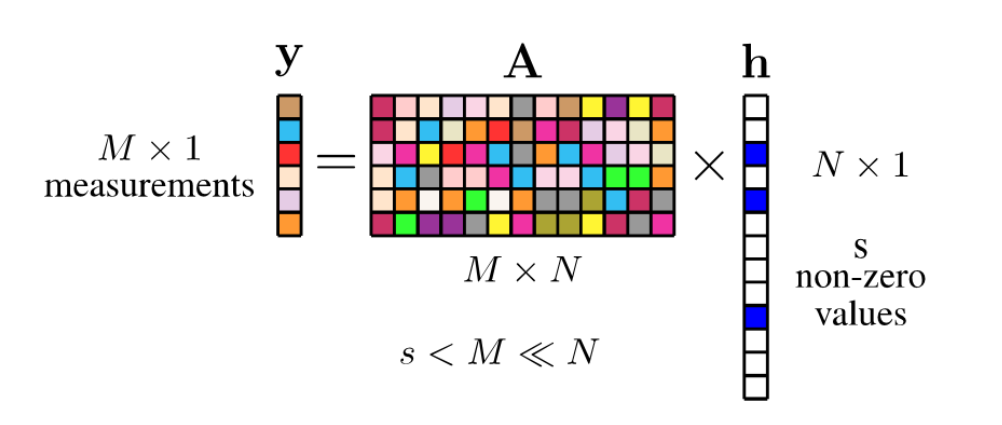
\includegraphics[width=0.8\textwidth]{cs-measurement.png}
    \label{fig:cs-measurement} \vspace*{-2mm}
    \caption{Illustration of sampling/measurement process in compressive sensing \cite{ref:Marques2019ReviewOfSparseRecovery}. The notation used here differs slightly from the notation adopted in this appendix (i.e., $\mathbf{A}$ and $\mathbf{h}$ in the figure correspond to $\mathbf{\Phi}$ and $\mathbf{x}$, respectively)}.
\end{figure}

In Section~\ref{sect:hetero-markov} of Chapter~\ref{chap:p2d}, we introduced a heterogeneous differential encoder which utilized deep compressive sensing networks. This appendix provides a brief overview of the relevant theory from compressive sensing based on the excellent survey \cite{ref:Marques2019ReviewOfSparseRecovery}.

Given a signal $\mathbf{x}\in\mathbb{R}^N$, denote a random measurement of this signal as 
\begin{align*}
    \mathbf{y} = \mathbf{\Phi}\mathbf{x}
\end{align*}
where $\mathbf{\Phi}\in\mathbb{R}^{M\times N}$ is referred to as the \emph{measurement matrix} and $\mathbf{y}\in\mathbb{R}^{M}$ is a low-dimensional measurement (i.e., $M << N$). The goal of compressive sensing is to recover the original signal $\mathbf{x}$ based on the low-dimensional measurement $\mathbf{y}$. The least-squares solution to this problem is given as
\begin{align}
    \min_{\hat{\mathbf{x}}}\|\hat{\mathbf{x}}\|_2 \; \text{subject to} \; \|\mathbf{y} - \mathbf{\Phi}\hat{\mathbf{x}}\|_2^2 < \epsilon \label{eq:undet-ls}
\end{align}
where $\epsilon > 0$ is some error tolerance. By construction, the matrix $\Phi$ has more columns than rows (i.e., $N >> M$), and consequently, the linear system (\ref{eq:undet-ls}) is underdetermined. Furthermore, the least-squares solution cannot return a sparse vector, and instead, the recovery of $\mathbf{x}$ is typically framed as a sparsity-constrained least-squares estimation problem, i.e.
\begin{align}
    \min_{\hat{\mathbf{x}}}\|\hat{\mathbf{x}}\|_0 \; \text{subject to} \; \|\mathbf{y} - \mathbf{\Phi}\hat{\mathbf{x}}\|_2^2 < \epsilon \label{eq:sparse-ls}
\end{align}
Under certain constraints, the original signal $\mathbf{x}$ can be perfectly reconstructed. However, this perfect reconstruction requires a combinatoric search over $\begin{pmatrix}N \\ s\end{pmatrix}$ (where $s$ is the number of non-zero elements in $\mathbf{x}$).
% \begin{align*}
%     \argmin_{\hat{\mathbf{x}}} \|\mathbf{y}-\mathbf{\Phi}\hat{\mathbf{x}}\|_2^2 + \lambda|\mathbf{\Phi}\mathbf{x}|_j.
% \end{align*}
Instead, the problem is often relaxed to use the $\ell_1$ norm,
\begin{align}
    \min_{\hat{\mathbf{x}}}\|\hat{\mathbf{x}}\|_1 \; \text{subject to} \; \|\mathbf{y} - \mathbf{\Phi}\hat{\mathbf{x}}\|_2^2 < \epsilon, \label{eq:lasso-ls}
\end{align}
which is referred to as the least absolute shrinkage and selection operation (LASSO). 

\section{The ISTA algorithm}
To solve the LASSO, it is possible to use proximal gradient methods from convex optimization \cite{ref:beck2009fast}. The gradient method that we focus on in this appendix is the iterative shrinkage threshold algorithm (ISTA), which is the namesake of the ISTANet algorithm discussed in Section~\ref{sect:hetero-markov} of Chapter~\ref{chap:p2d}. For the $\ell_1$ regularized problem, gradient-based methods solve 
\begin{align*}
    \min \left\{f(\mathbf{x})+\lambda\|\mathbf{x}\|_1\right\}
\end{align*}
using the iterative steps
\begin{align*}
    \mathbf{x}_k &= \argmin_{\mathbf{x}} \left\{f(\mathbf{x}_{k-1}) + \langle \mathbf{x} - \mathbf{x}_{k-1}, \nabla f(\mathbf{x}_{k-1}) \rangle + \frac{1}{2t_k}\|\mathbf{x} - \mathbf{x}_{k-1}\|^2 + \lambda\|\mathbf{x}\|_1\right\} \\
    &= \argmin_{\mathbf{x}} \left\{\frac{1}{2t_k}\|\mathbf{x} - (\mathbf{x}_{k-1} - t_k\nabla f(\mathbf{x}_{k-1}))\|^2 + \lambda\|\mathbf{x}\|_1\right\},
\end{align*}
where $t_k>0$ is the stepsize for the algorithm. Note that the second line is admitted by ignoring the constant terms. The $\ell_1$ term is separable, and consequently, computing the iteration $\mathbf{x}_k$ can be done by solving a one-dimensional minimization problem for each component of $\mathbf{x}_k$,
\begin{align*}
    \mathbf{x}_k &= \mathcal{T}_{\lambda t_k} (\mathbf{x}_{k-1} - t_k\nabla f(\mathbf{x}_{k-1})).
\end{align*}
Note the shrinkage operator, $\mathcal{T}_{\alpha} : \mathbb{R}^n \to \mathbb{R}^n$,
\begin{align*}
    \mathcal{T}_{\alpha}(\mathbf{x})_i &= \text{soft}(x_i, \alpha) = (|x_i| - \alpha)_{+}(x_i)
\end{align*}
\begin{figure*}[!hbtp]
\centering
\def\svgwidth{0.8\linewidth}
\input{images/soft-threshold.pdf_tex}
\caption{Soft-threshold function used in the ISTA algorithm.}
\label{fig:soft_threshold}
\end{figure*}
When this gradient method is applied to the compressive sensing problem, we have $f(\mathbf{x}) := \|\mathbf{\Phi}\mathbf{x}-\mathbf{y}\|$, and the resulting iterative algorithm is known as ISTA, where the iterations take the form,
\begin{align}
    \mathbf{x}_k &= \mathcal{T}_{\lambda t_k}(\mathbf{x}_{k-1} - t_k\mathbf{\Phi}^T(\mathbf{\Phi} \mathbf{x}_{k-1} - \mathbf{y}))
\end{align}
These iterations of the ISTA algorithm correspond to the gradient step and the proximal step of (\ref{eq:istanet-grad}) and (\ref{eq:istanet-prox}) for ISTANet+ (see Chapter~\ref{chap:p2d}, Section~\ref{sect:hetero-markov}). Note that ISTANet+ differs from the vanilla formulation of ISTA in a few key ways, namely:
\begin{itemize}
    \item \textbf{Learnable sparse basis}: ISTANet+ assumes that the $\ell_1$ penalty term is imposed on a sparse transform of the input data (i.e., $\|\mathbf{\Psi}\mathbf{x}\|_1$). Furthermore, the sparse transform and its inverse (i.e., $\mathbf{\Psi}$ and $\mathbf{\Psi}^{-1}$) are learned using convolutional layers (i.e., $\mathcal{G}$ and $\tilde{\mathcal{G}}$), and the `soft' operator is applied to sparse transform.
    \item \textbf{Residual connections}: ISTANet+ uses the sparse transform and the `soft' operator on the residual of the estimate rather than the estimate itself.
\end{itemize}